\subsection{Orbitals}
\begin{minipage}{0.43\columnwidth}
    \textbf{Orbital Energies}
    \begin{center}
        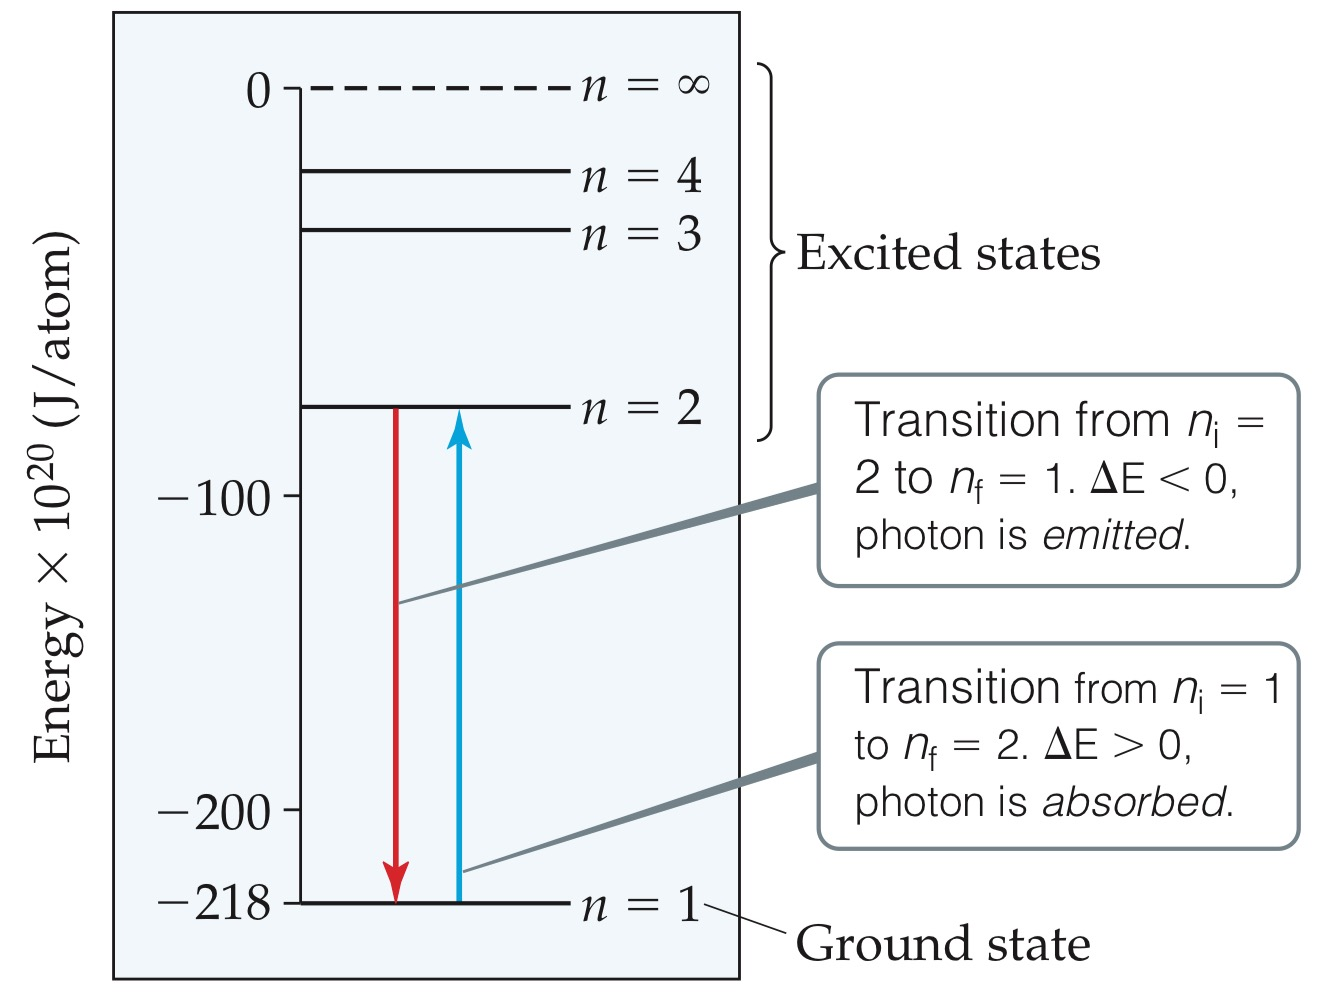
\includegraphics[width = \linewidth]{images/energy_transition_.jpeg}
       
    \end{center}
     \textbf{Quantum Numbers}
    \begin{enumerate}[leftmargin=0.20cm, itemsep=0.05pt]
        \item Principial Quantum Number $n$ (1, 2, 3, ...)
        \item Angular Quantum Number $L$ : [0, n-1],\\
        $0 \equiv$ s, $1 \equiv$ p, $2 \equiv$ d, $3 \equiv$ f
        \item Magnetic quantum Number $m_e$ $[-L, L]$
        \item Spin Magnetic Quantum Number $m_s$ ($-\frac{1}{2}$ or $\frac{1}{2}$)
    \end{enumerate}
    \textcolor{red}{\textbf{Pauli Exclusion Principle}}\\
\fbox{\begin{varwidth}{\textwidth}
\centering
No two electrons in an atom can have the \\ same set of four quantum numbers $n, L, m_e, m_s$
\end{varwidth}}   
 
\end{minipage}
\begin{minipage}{0.56\columnwidth}
    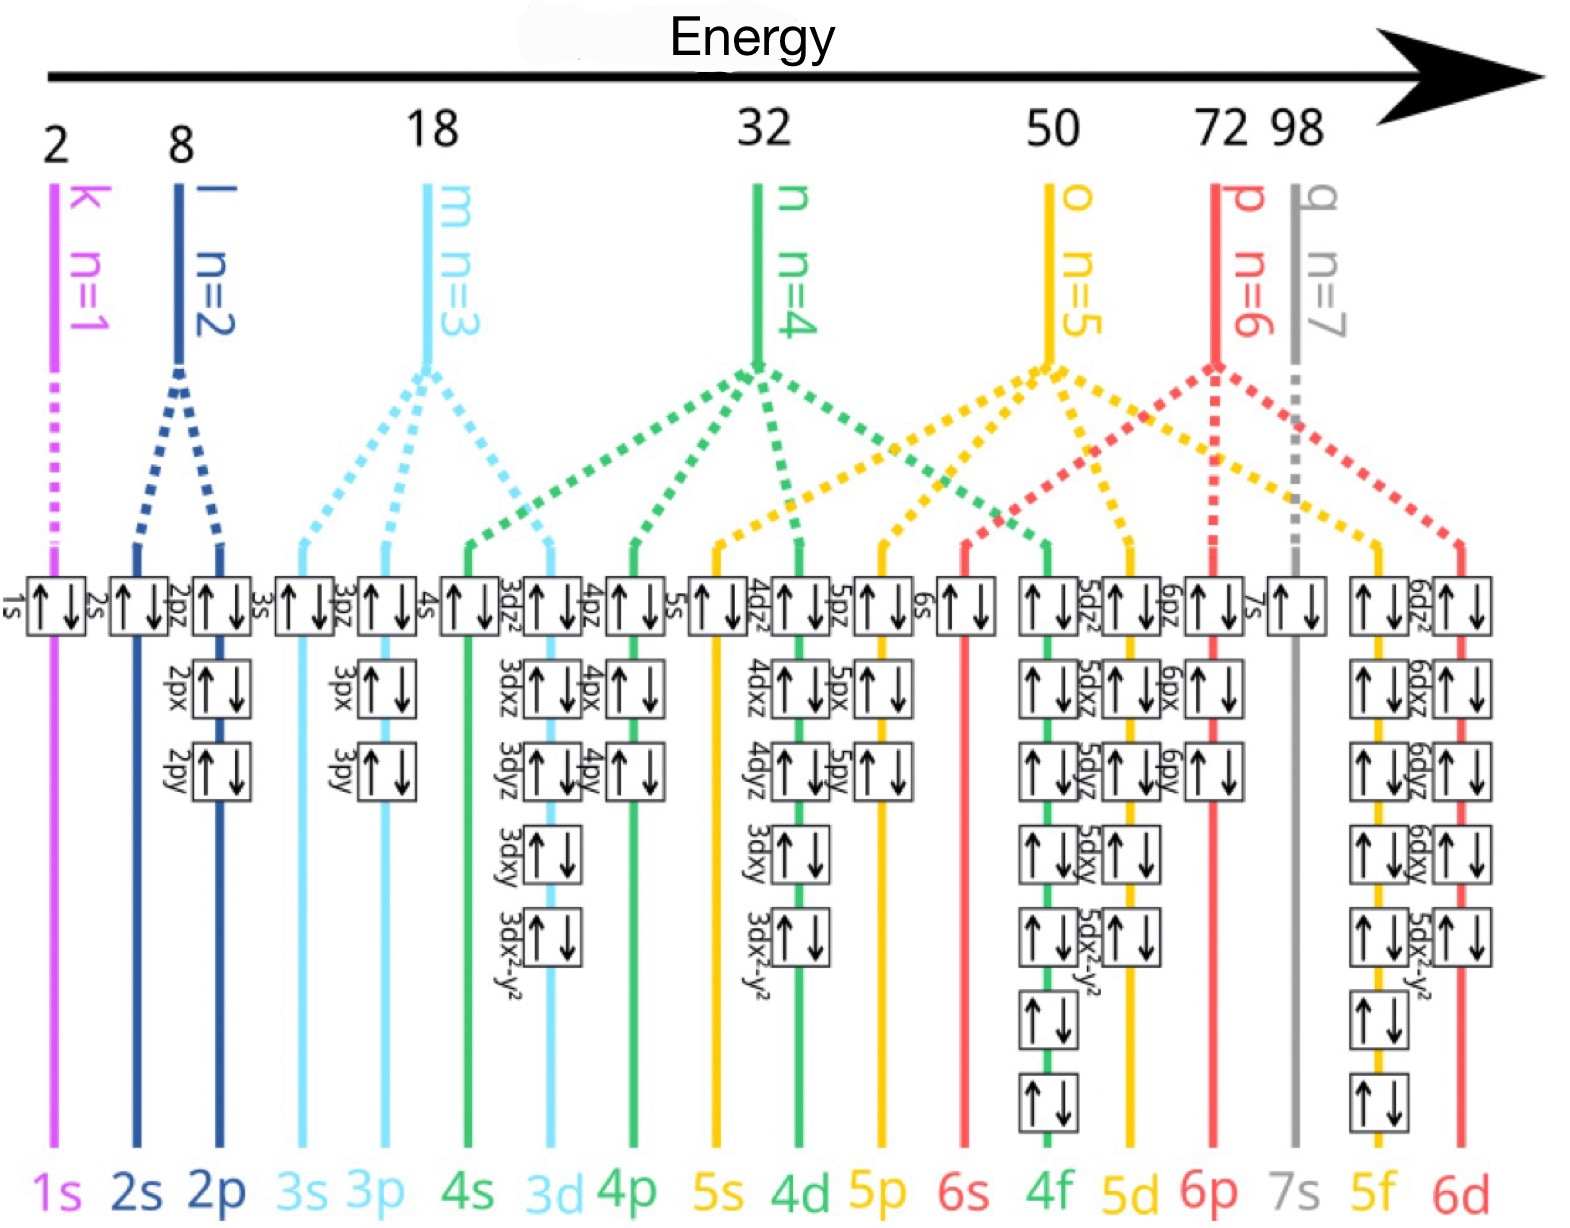
\includegraphics[width = 0.8\linewidth]{images/Orbitals.jpeg}
     \begin{minipage}{0.7\linewidth}
         \begin{center}
             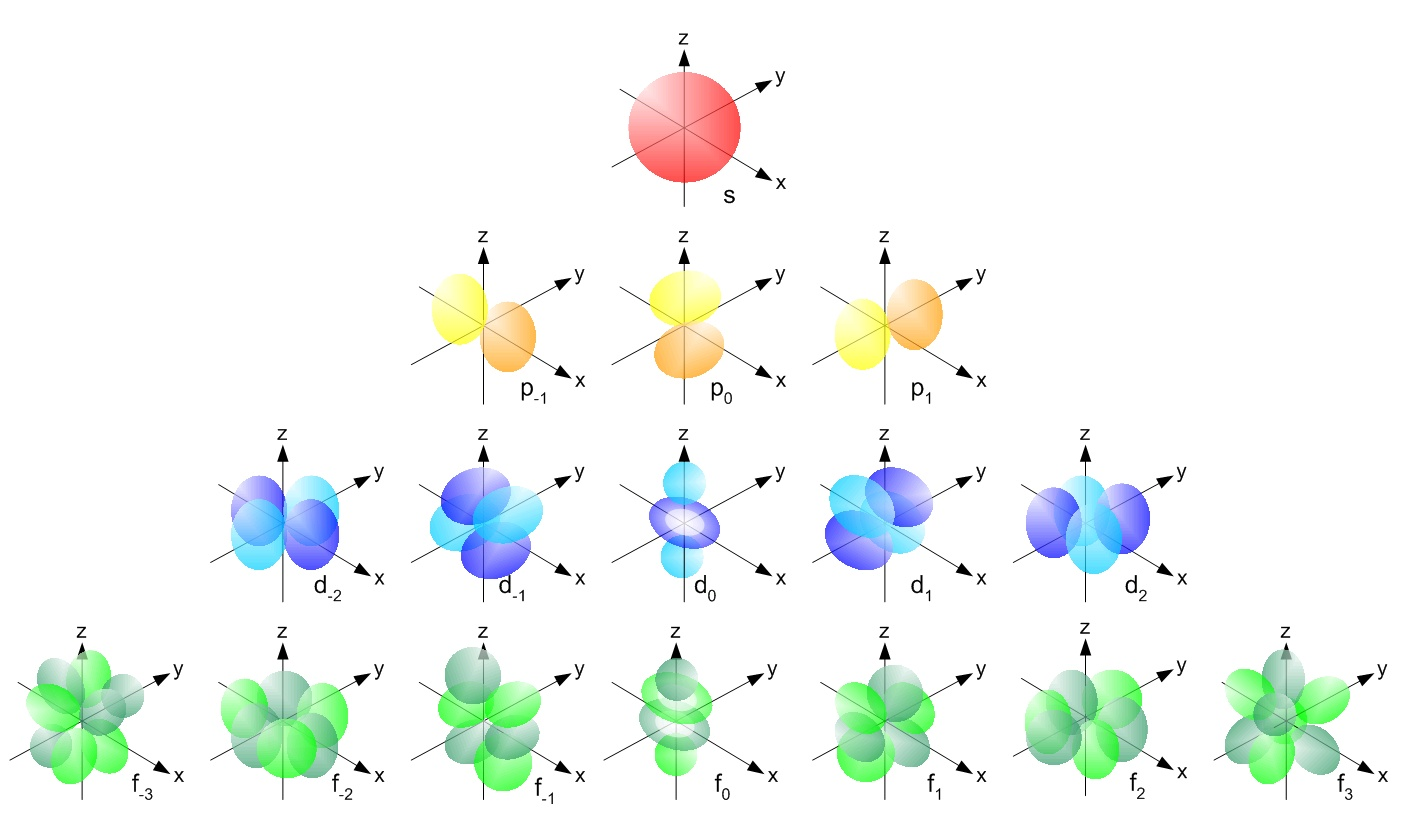
\includegraphics[width = \linewidth]{images/orbital_shapes.jpg}
         \end{center}
     \end{minipage}\\
    \textcolor{red}{\textbf{Hund's Rule}}\\
    \fbox{\begin{varwidth}{\textwidth}
    \centering
    When filling degenerate orbitals the lowest energy is\\ attained when the number of electrons having the same spin is maximized
    \end{varwidth}}  
\end{minipage}

\begin{minipage}{0.60\columnwidth}
    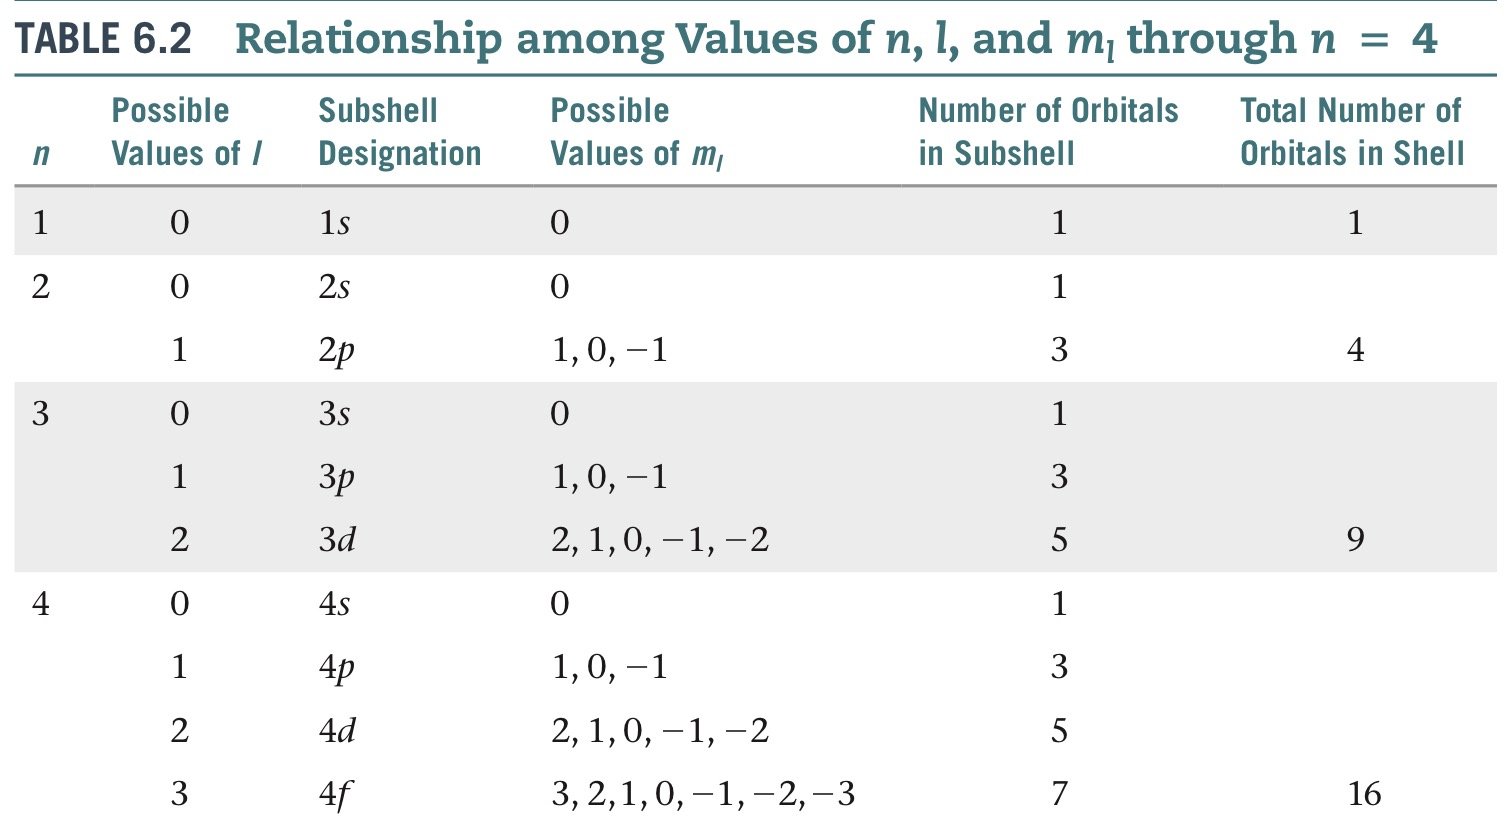
\includegraphics[width = \linewidth]{images/Quantum_numbers_up_to_n_4.jpeg}
\end{minipage}
\begin{minipage}{0.37\columnwidth}
    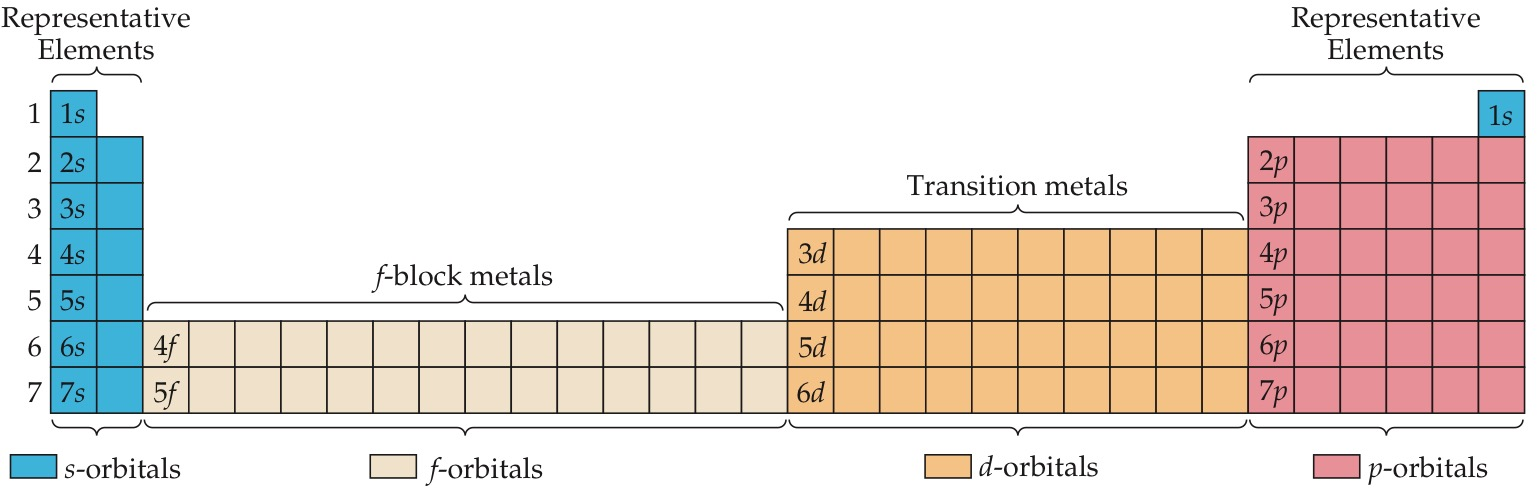
\includegraphics[width = \linewidth]{images/PSE_Quantum_Numbers.jpeg}
    \begin{itemize}
        \item s-orbital: sphere-like
        \item p-orbital: dumbbell-like
        \item d-orbital: usually 4-leafed clover
        \item f-orbital: 2x2 rounded Rubik's cube/other complicated shapes 
    \end{itemize}
\end{minipage}

